% This is samplepaper.tex, a sample chapter demonstrating the
% LLNCS macro package for Springer Computer Science proceedings;
% Version 2.20 of 2017/10/04
%
\documentclass[runningheads]{llncs}
%
\usepackage{graphicx,amsfonts,algorithm,algorithmic,multirow,amsmath,xcolor,bm,makecell,balance,subfigure,caption}
% Used for displaying a sample figure. If possible, figure files should
% be included in EPS format.
%
% If you use the hyperref package, please uncomment the following line
% to display URLs in blue roman font according to Springer's eBook style:
% \renewcommand\UrlFont{\color{blue}\rmfamily}

\begin{document}
%
\title{PROPER:a Tool for Analyzing Termination and Assertions for Affine Probabilistic Programs}
%
%\titlerunning{Abbreviated paper title}
% If the paper title is too long for the running head, you can set
% an abbreviated paper title here
%
\author{Xuhui Zhao\inst{1}\orcidID{0000-1111-2222-3333} \and
Yuxin Deng\inst{2}\orcidID{1111-2222-3333-4444} \and
Hongfei Fu\inst{3}\orcidID{2222--3333-4444-5555}}
%
\authorrunning{F. Author et al.}
% First names are abbreviated in the running head.
% If there are more than two authors, 'et al.' is used.
%
\institute{East China Normal University, Shanghai, China \\ \email{51184501088@stu.ecnu.edu.cn} 
\and East China Normal University, Shanghai, China \\ \email{yxdeng@sei.ecnu.edu.cn}
\and Shanghai Jiao Tong University,  Shanghai, China \\ \email{fuhf@cs.sjtu.edu.cn}}
%
\maketitle              % typeset the header of the contribution
%
\begin{abstract}
Probabilistic programs combine probabilistic reasoning models with Turing complete programming languages, unify formal descriptions of calculation and uncertain knowledge, and can effectively deal with complex relational models and uncertain problems. In this paper, we provide a tool for analyzing termination and assertions for affine probabilistic programs, PROPER. On one hand, it can help to analyze the termination property of affine probabilistic programs both qualitatively and quantitatively. It can check whether a probabilistic program terminates with probability $1$, estimate the upper bound of expected termination time, and calculate the number of steps after which the termination probability of the given probabilistic program decreases exponentially.  On the other hand, it can estimate the correct probability interval for a given assertion to hold, which helps to analyze the influence of uncertainty of variables on the results of probabilistic programs. Our work is implemented and the effectiveness of PROPER is demonstrated through various affine probabilistic programs.

\keywords{Probabilistic Programming  \and Program Verification \and Termination \and Ranking Supermartingale.}
\end{abstract}
%
%
%
\section{Introduction}
In traditional precise logic, the representation and reasoning of knowledge is mechanical and deterministic, just like Demon de Laplace, capable of inferences about the future based on the known facts. But in real world, there are a large number of uncertainty problems , which require us to use prerequisite knowledge and deductive reasoning to predict the results, that is to say, to make decisions on nondeterministic problems through probabilistic reasoning. Probability is an important tool for the representation of imprecise and incomplete knowledge. Therefore, probabilistic programs are put forward for that purpose. 

Probabilistic programs are a kind of logic programs with probabilistic facts. Probabilistic programs are often used to build generation models and reason about its hidden process. They make probabilistic reasoning models easier to build and can estimate the possibilities of certain events to occur. They can also be used to quantify the uncertainty in the prediction instead of predicting a single value. Several practical probabilistic programming languages(such as Edward~\cite{tran2016edward}, Anglican~\cite{Dav2016Design}, WebPPL~\cite{Noah2014language} and Church~\cite{Noah2008language}) now exist, they can build powerful models and are used in a wide range of applications, such as business, military, scientific research and daily life. Probability is becoming more and more important in actual calculations, such as risk analysis, medical decision-making, differential privacy mechanisms, etc. With the increasing demand for high confidence software, the analysis and verification of probabilistic programs has also received widespread attention in academia and industry. Therefore, our work is a valuable and challenging, which the reliability and stability of the program can be better guaranteed. Program verification is an incalculable problem in computer theory. In view of this difficulty, a realistic consideration is that we only verify those properties that are more important and can be verified automatically. In the current work, we present PROPER, a tool for probabilistic program verification, namely, analyzing termination and assertions for affine probabilistic programs (probabilistic programs whose all arithmetic expressions are linear). The tool builds on \cite{kris2016termination,cha2015algorithmic,Sankaranarayanan2013Static}. 

Currently, due to the demand for high-confidence software, verification of program termination is an important part of software design and development. Termination analysis is an important part of software complete correctness. Failure to terminate the program may cause the system to become unresponsive, resulting in system failure. For termination analysis, our goal is to analyze the termination property of a given affine probabilistic program qualitatively and quantitatively. The qualitative analysis aims to answer whether an affine program terminates with probability $1$ (almost-sure termination). The quantitative analysis aims to approximate the expected termination time (expectation problem) and compute a bound $N$ such that the probability to terminate after $N$ steps decreases exponentially (concentration problem). The method we adopt is to synthesis of polynomial ranking supermartingales, which is an extension of linear ranking-supermartingale. 

For assertion analysis, our goal is to estimate the correct probability interval of the assertion that meets the given specifications in an affine probabilistic program. It has great potential value in artificial intelligence fields such as incomplete knowledge processing systems, meta-reasoning, cognitive query, and conformant probability planning. The main application scenarios include fuzzy information description, incomplete information for reasoning or noise in information. We observe that for probabilistic programs, by selecting a finite set of appropriate paths, facts about the behavior of the entire program can be derived. Therefore, we used the static analysis method for probabilistic programs that can perceive, manipulate and control based on uncertain data. Firstly, We select a finite set of adequate program paths through certain strategies for estimating probability bounds. Then evaluate each path through symbolic execution and probabilistic volumebound calculations. The sum of interval boundaries generated by each path is the probability of assertion for the program as a whole.

To summarize, this paper makes the following contributions:
\begin{enumerate}
	\item Defining and parsing probabilistic programs. More than ten kinds of probability distributions are built in, which is convenient to be called to build probabilistic models.
	\item Reducing the termination analysis of a given program to a linear programming problem. We also consider the concentration results under the premise that the program is terminating.
	\item Reducing the estimation of a given assertion to a polyhedron solving problem. In particular, it can handle probabilistic programs with infinitely many states.	
\end{enumerate}

The source code and the experimental data given in this paper are all available in the repository \url{https://github.com/Healing1219/PROPER}.

\section{Preliminaries}
Probabilistic programs is extending classical imperative programs, which can be constructed by generating integer and real random values according to a fixed set of distributions. In this subsection, we illustrate the syntax and semantics of affine probabilistic programs that we study.

\begin{figure}[ht]
	\centering
	\begin{tabular}{rcl}
		\hline
		% after \\: \hline or \cline{col1-col2} \cline{col3-col4} ...
		program & $:=$ & typeSpecifier main\{stmt$^*$\} \\
		stmt & $:=$ & assign $\mid$ condStmt $\mid$ while \\
		assign & $:=$ & intAssign $\mid$ realAssign \\
		condStmt & $:=$ & ifStmt $\mid$ ifElseStmt\\
		while & $:=$ & while (test) stmt$^*$\\
		intAssign & $:=$ &  intVar = intConst $\mid$ intVar $\sim$ intRandom\\
		realAssign & $:=$ & realVar = realConst $\mid$ realVar $\sim$ realRandom\\
		intRandom & $:=$ & uniformInt(intConst, intConst)\\
		&  & | Bernoulli(intConst, intConst)\\
		&  & $\cdots$ \\
		realRandom & $:=$ & uniformReal(realConst, realConst)\\
		&  & | Gaussian(realConst, realConst)\\
		&  & $\cdots$ \\
		intExpr & $:=$ & intConst $\mid$ intRandom $\mid$ intExpr $\pm$ intExpr\\
		& & intConst* intExpr $\mid$ intExpr / intConst\\
		realExpr & $:=$ & realConst $\mid$ realRandom $\mid$ realExpr $\pm$ realExpr\\
		& & realConst* realExpr $\mid$ realExpr / realConst\\
		boolExpr& $:=$ & true $\mid$ false $\mid$ boolExpr $\wedge$ boolExpr \\
		& & intExpr relop intExpr $\mid$ realExpr relop realExpr\\
		relop & $:=$ & <  $\mid$  > $\mid$ $\geq$ $\mid$ $\leq$ $\mid$ ==\\
		\hline
	\end{tabular}
	\caption{Syntax specification of a probabilistic language}	\label{syntax}
\end{figure}

\textbf{Syntax.} In order to analyze and verify probabilistic programs, we first need a probabilistic language sufficiently expressive and easy to understand. We define a probabilistic language, whose syntax specification is shown in Figure~\ref{syntax}. The statements in the probabilistic language are similar to those in classic imperative languages, mainly composed of three types of statements: assignment, condition-branch (if-else) and loop statements (while). The main difference is that we now have a collection of random value generators (discrete distribution, Binomial distribution, Poisson distribution, Integer Uniform distribution, Real Uniform distribution, Exponential distribution, Gamma distribution, Beta distribution, Geometric distribution), which can be used to simulate different probability distributions. Variables are classified into two types: program variables $X$ and sampling variables $R$. Program variables are ordinary variables that can be assigned to integer, real, boolean variables or arithmetic expressions. Boolean variables are mainly used for condition-branch and loop statements. Sampling variables are assigned with dynamically generated values when the program is running, which is subject to a continuous or discrete probability distribution. The values may be different each time. In addition, assertion expressions also have certain specifications. The format of assertions is a Boolean expression that contains variables. In the case of compound conditions, we also support logical operators ``and''(\&\&) in assertion expressions.

\textbf{Sematics.} We use control flow graphs (CFGs) to express the semantics of probabilistic programs, which we difine below: 

Formally, a CFG is a tuple in the form $(L,X,R,\mapsto,\bot)$, where:
\renewcommand{\labelitemi}{$\vcenter{\hbox{\tiny$\bullet$}}$}
\begin{itemize}
	\item $L$ is a finite set of labels $L=\{\ell_0,\ell_1,\dots,\ell_n\}$ used to represent control locations. Each statement in a program has a unique label. For example, $\ell_0$ usually indicates the starting location.
	%, $\ell$$_n$ indicates the last location.
	
	\item $X=\{x_0,\dots,x_n\}$ is a set of program variables and $R=\{r_1,\dots,r_m\}$ is a set of sampling variables.
	
	\item $\mapsto$ is a transition relation. Its element is in the form $(\ell,\alpha,\ell')$, representing one step of transition from control location $\ell$ to $\ell'$, by an update function $\alpha$: $\mathbb{R}^{|X\cup R|}\to \mathbb{R}^{|X|}$.
	
	\item $\bot$ is a sign of the exit of the program.
\end{itemize}

Obviously, any probabilistic program can be transformed to a CFG naturally. Each label represents the control location in the execution of the probabilistic program, where the statement of the control location is the next program position to be executed, as show in right of Figure~\ref{example1}. 
The following, we assume that the probabilistic program P with two linear sequences $X=\{x_0,\dots,x_{n}\}$ and $R=\{r_0,\dots,r_{|m|}\}$, interpreting each vector $x \in \mathbb{R}^{|X|}$ as a program variable and $r \in \mathbb{R}^{|R|}$ as a sampling variable. And let $(L,X,R,\mapsto,\bot)$ is the CFG associated with the probabilistic program P. For notational convenience we assume the configuration is a tuple $(\ell, x)$, where $\ell$ is a location of P and $x$ is a valuation of program variables. We fix $(\ell_0, x_0)$ to be the initial configuration of the program P. The program updates its state according to the transition relation. The transition relation $(\ell,\alpha,\ell')$ specifies the transitions between labels together with the additional information specific to different types of labels. They also can be viewed as a set $f=\{f_0,\dots,f_{|n|}\}$, where each $f_i$ denotes $\mathbb{R}^{|X \cup R|} \to \mathbb{R}$. The execution of P is an infinite sequence of configurations whose each finite prefix is a finite path $(\ell_0, x_0) \dots (\ell_k, x_k)$. For each $0\leq i\leq k$, enable the transition relation $(\ell_i, f, \ell_{i+1})$ in $(\ell_i, x_i)$, and evaluate the random variable r so that $x_{i+1}=f(x_i,r)$. If there is a finite path starting from $(\ell_0, x_0)$ and ending with $(\ell_k, x_k)$, you can access the configuration $(\ell_k, x_k)$ from the starting configuration $(\ell_0, x_0)$. According to the different types of statements, the transition relation of each label can be divided into the following situations. Suppose the current configuration is $(\ell_i, x_i)$.
\renewcommand{\labelitemi}{$\vcenter{\hbox{\tiny$\bullet$}}$}
\begin{itemize}
	\item  Assignment Statements: for $x:=exp$, where $x$ is a variable and $exp$ is an arithmetic expression or constant. Through the transition $(\ell, f(x,exp), \ell')$, the configuration of P transit to $(\ell_{i+1}, x_{i+1})$, where $x_{i+1} = f(x_i,r)$
	\item  Conditional-branch Statements: For $\textbf{if}$ $\phi$ $\ell_a$ $\textbf{else}$ $\ell_b$, $x_{i} = x_{i+1}$, if the value of $\phi$ is true($x_i \models f$), the configuration of P transit to $(\ell_a, x_a)$, otherwise $(\ell_b, x_b)$.
	\item  Loop Statements: For $\textbf{while}$ $\phi$ $\textbf{do}$ $\ell_{i+1}$, if the value of $\phi$ is true($x_i \models f$), the configuration of P transit to $(\ell_{i+1}, x_{i+1})$, otherwise $(\ell_{out}, x_{out})$, where $\ell_{out}$ means out of the loop.
	\item  Location of termination: $\ell_{i+1} =\ell_{i}=\bot$ marks the end of P, and $x_{i} = x_{i+1}$
\end{itemize}

\begin{figure}[htbp]
	\vspace{-0.5cm}  %调整图片与上文的垂直距离
	\centering %居中
	\subfigure{ %第一张子图
		\begin{minipage}{4cm}
		\centering %子图居中
		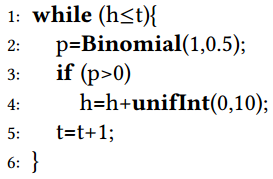
\includegraphics[scale=0.8]{img/ex1} 
		%\subfigcapskip=-5pt
		\setlength{\belowcaptionskip}{-14cm}
		\end{minipage}
	}
	\subfigure{ %第二张子图
		\begin{minipage}{6cm}
		\centering %子图居中
		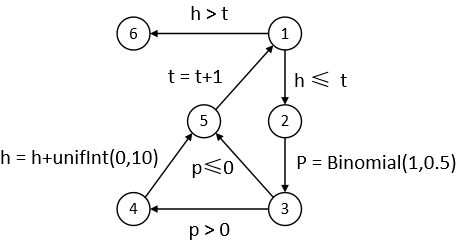
\includegraphics[scale=0.9]{img/CFG1} 
		\end{minipage}
	}
	\caption{A probabilistic program with its CFG} % %大图名称
	\label{example1} %图片引用标记
	%\setlength{\belowcaptionskip}{-3cm}   %调整图片标题与下文距离
\end{figure}

\paragraph{Example 1} In Figure~\ref{example1}, we show a probabilistic program on the left and its control flow graph on the right. In the program,  $t$ is a program variable,  $p$ and $h$ are smapling variables. Here, two probability distributions are used: \textbf{Binomial}(1,0.5) represents a binomial distribution, which yields values 0 and 1 with equal probability; \textbf{unifInt}(0,10) represents an integer uniform distribution, which yields the integers between 0 and 10  with equal probability. The numbers 1-6 on the left are the program control locations, where 1 is the starting location and 6 is the terminal location. The probabilistic program simulates a scene of the tortoise hare race. The tortoise's initial position is $t$ and the hare's initial position is $h$.  The tortoise  always moves at the speed of 1. When $p>0$,that is to say, there is a probability of 0.5, the hare increases its speed by a random number between 0 and 10. The program terminates when the hare passes the tortoise.

\iffalse
\newcommand{\tabincell}[2]{\begin{tabular}{@{}#1@{}}#2\end{tabular}}
\begin{table}[htb]
	\caption{Specification of the inbuilt random value generators}
	\label{distribution}
	\begin{tabular}{lll}  
		\toprule   
		Name & Parameter & \makebox[4cm][c]{Density Function} \\  
		\midrule   
		R($\mathbb{X},\mathbb{P}$) & $\sum\limits_{n=1}^N p_n$=1 & $P(X=x_k)=p_k$\\  
		Binomial(n,p) & \tabincell{c}{0<p<1\\n$\geq$1} &$\tbinom{k}{n}p^k(1-p)^{n-k}, k=1,2,\dots$ \\  
		Poisson($\lambda$) & $\lambda$>0 &$\frac{\lambda^ke^{-\lambda}}{k!}$ \\   
		UnifInt(a,b) & a$\leq$b & 
		$\left\{
		\begin{array}{lr}
		\frac{1}{b-a} &, b>a \\
		1 & ,a=b\\
		\end{array}
		\right.$ \\
		UnifReal(a,b) & a<b & $\frac{1}{b-a}$ \\  
		Exponential($\theta$) & $\theta$>0 & $\frac{1}{\theta}e^{\frac{x}{\theta}}$ \\    
		Normal($\mu$,$\sigma^2$) &$\sigma$>0 &$\frac{1}{\sqrt{2\pi}\sigma}e^{-(x-\mu)^2/(2\sigma^2)}$ \\
		Gamma($\alpha$,$\beta$) & $\alpha, \beta$>0 & 
		$\frac{1}{\beta^\alpha\Gamma(\alpha)}x^{\alpha-1}e^{\frac{-x}{\beta}} , x>0 $  \\  
		Beta($\alpha$,$\beta$) & $\alpha, \beta$>0 & $\frac{\Gamma(\alpha+\beta)}{\Gamma(\alpha)\Gamma(\beta)}x^{\alpha-1}(1-x)^{\beta-1}$,0<x<1\\    
		Laplace(x|$\mu,\lambda$) & $\lambda>0$ &$\frac{1}{2\lambda}e^{\frac{|x-\mu|}{\lambda}}$ \\
		Geometric(p) & 0<p<1 & $(1-p)^{k-1}p, k=1,2,\dots$ \\     
		T(n) &n$\geq$1 &$\frac{\Gamma(\frac{n+1}{2})}{\sqrt{n\pi}\Gamma(\frac{n}{2})}(1+\frac{x^2}{n})^{-(n+1)/2}$ \\
		\bottomrule  
	\end{tabular}
\end{table}
\fi

\section{Architecture Design }
\begin{figure}[h]
	\centering
	\label{architecture}
	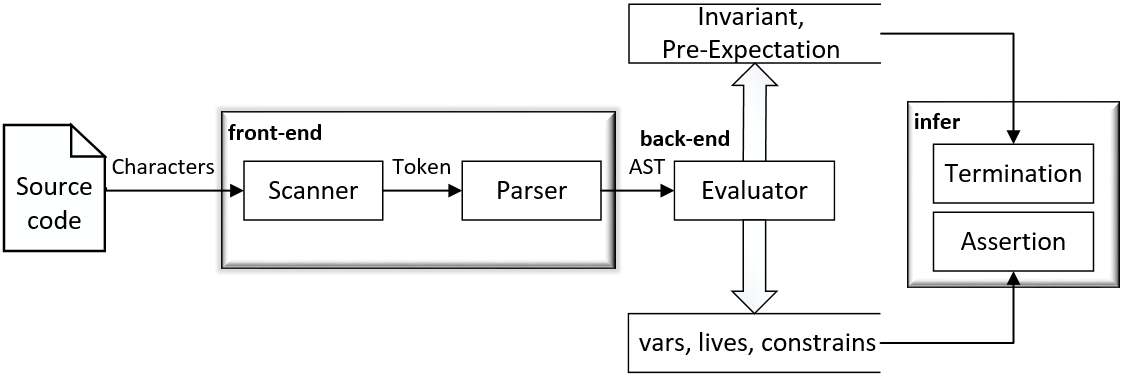
\includegraphics[scale=0.6]{img/architecture}
	\caption{The architecture of PROPER}
\end{figure}
PROPER's architecture is mainly composed of three parts: front-end, back-end and infer, as shown in Figure \ref{architecture}.  

Front-end and back-end can be regarded as a whole, based on the interpreter, which converts the source code into some effective intermediate representations and executes them line by line. The front-end work content is similar to the compiler front-end, mainly including scanner and parsers. Generally, scanner input the source code and coverts it into token stream. This process is called lexical analysis. Then the output of the scanner is used as the input of parser, which is used to construct the abstract syntax tree.
In this process, the symbol table is created. It is essentially a database, which is used to store related information such as variables and function calls. It needs four features: high speed, easy maintenance, flexibility and repeatability. In order to meet the above requirements, we use a chain hash table structure to achieve, which helps to quickly and effectively insert new data nodes, access and update existing data nodes. The average time complexity of insertion and deletion is $O(1)$. The specific structure is shown on the right side of Figure \ref{symbolTable}.
\begin{figure}[h]
	\centering
	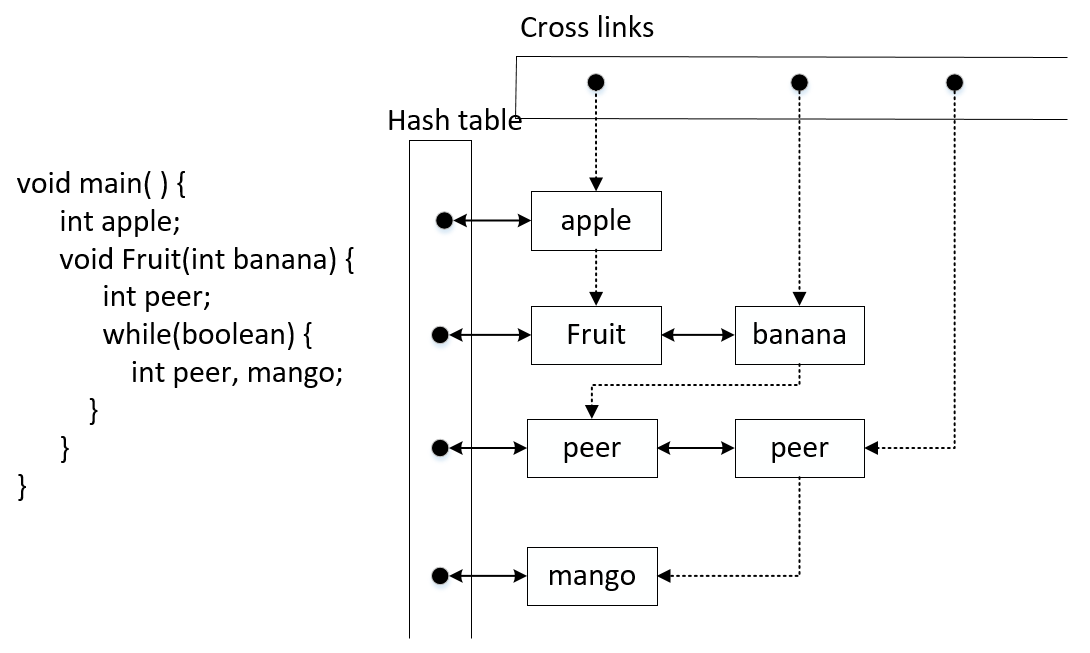
\includegraphics[scale=0.6]{img/symbolTable}
	\caption{Data Structure of the Symbol Table}
	\label{symbolTable}
\end{figure}

All variables are stored in a hash table, and variables hashed to the same location are connected by a double linked list, thus solving the problem of supporting repeatability. An example is shown on the left side of Figure \ref{symbolTable}. The linked list at the top is used to store the starting pointers of variables at different levels. Here, the global variables ``apple" and the function name ``Fruit" belong to the first-level variables, ``banana" and ``peer" belong to the second-level variables, and ``peer" and ``mango" belong to the third-level variables. Because the variable name is used for hashing, the same variable name ``peer" is hashed to the same location. Similarly, different variable names may also be hashed to the same location. We assume that ``banana" is hashed to the same location as ``Fruit", and the same level is connected by a linked list.

The back-end executes the code according to the abstract syntax tree. It will recursively traverse each child node. Each non-terminal symbol corresponds to such a node, the structure of the node is shown in Figure \ref{class}(b). ``parent" and ``children" correspond to the parent node and child node list respectively; ``value" and ``text" are used to store the parsed value and text information of the symbol; ``type" is the type of non-terminal, such as ``STMT", ``EXPR",``UNARY", etc.; ``production" corresponds to the sequence number of the parsed syntax expression. And ``symbol" corresponds to the record in the symbol table, the structure is shown in Figure~\ref{class}(a). ``name" is the name of the symbol,; ``level" represents the level of the variable; ``duplicate" indicates whether it is a variable with the same name. If the symbol corresponding to the function name, ``args" points to the function parameters list, and ``next" points to the next variable symbol at the same level.

\begin{figure}[htbp]
	%\vspace{-0.5cm}  %调整图片与上文的垂直距离
	\centering %居中
	\subfigure[]{ %第一张子图
		%\begin{minipage}{5cm}
		\centering %子图居中
		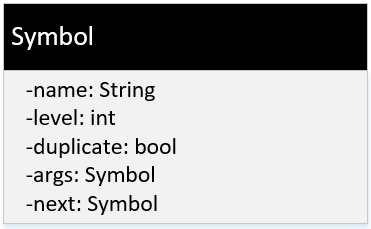
\includegraphics[scale=0.8]{img/symbol} 
		%\end{minipage}
	}\hfill
	\subfigure[]{ %第二张子图
		%\begin{minipage}5cm}
		\centering %子图居中
		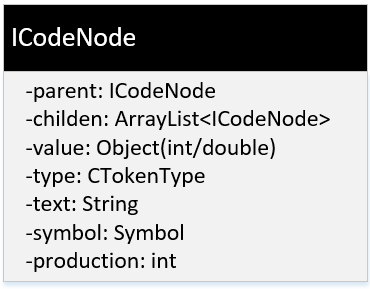
\includegraphics[scale=0.75]{img/icodenode} 
		%\end{minipage}
	}
	\caption{The internal structure of ``Symbol" and ``ICodeNode" class} % %大图名称
	\label{class} %图片引用标记
	%\setlength{\belowcaptionskip}{-1cm}   %调整图片标题与下文距离
\end{figure}

While executing the syntax tree, we also collect the relevant information for inferring.
For termination analysis, we need invariant and Pre-Expectation, which we will introduce these two concepts in detail in section 4. For assertion analysis, we need vars, lives, and constraints of each path. Vars is the set of variables included in the program; lives is the set of variables involving the assertion, used for path slice; constraints are related constraints. 

\section{Termination Analysis}
Termination analysis is an important part of program verification. If a loop program terminates for all initial values that can enter the loop, the program is said to be terminating.  Ensuring termination is a necessary condition for many properties of programs such as total correctness. 

Generally speaking, the termination of a program is undecideable~\cite{Turing1936On}, but for some subclasses of programs, the termination can be verified. In this paper, we prove the termination of the affine probabilistic programs by synthesizing ranking supermartingales~\cite{Chakarov2013Martingales}. We first extend the traditional linear ranking supermartingale concept to polynomial ranking supermartingales, and verify the termination of the affine probability program by synthesizing polynomial rank supermartingales. PROPER implements Algorithm \ref{TA}~\cite{kris2016termination,cha2015algorithmic} to analyze probabilistic termination qualitatively and quantitatively. 

\paragraph{Qualitative analysis} It mainly analyzes whether a probabilistic program will terminate with probability $1$(almost sure termination).
To better understand the following content, we need to comprehend the concept of polynomial ranking supermartingale, invariants and pre-expectation.
\begin{enumerate}
	\item[-] \textbf{Invariant} is a function $I$ that assigns a set $I(\ell)$ on variables $X$ to each label $\ell$. Thus for all configurations $(\ell,x)$ that can be reachable from the initial configurations $(\ell_0, x_0)$ by running the program, it will hold that $x \models I(\ell)$. In PROPER, we only support linear invariants, which can be represented by a finite number of linear inequalities.
	\item[-] \textbf{Pre-Expectation} is about the expression over the variables across a transition $\mapsto$, the specific calculation formula can refer to step 2.2 of  Algorithm \ref{TA}. Intuitively, pre-expection is the expected value of polynomial ranking  supermartingale $g(\ell,\cdot)$ in the next step of program execution.
	\item[-] \textbf{Polynomial Ranking Supermartingale}~\cite{Chakarov2013Martingales}(pRSM) is a collection of functions at each label, represented by the template $g(\ell,\cdot)$ with the maximal degree $d$. It satisfies $pre(\ell,x)\leq g(\ell,x)-\varepsilon$ and $g(\ell,x)\geq 0$ at non-terminal location. $g(\ell,x)=K$ at terminal location, where $K\leq -\varepsilon$ and $\varepsilon\geq 0$. The dividing line between termination and non-termination is 0, that shows each function is non-negative at non-terminal location. So this method can not handle the distribution without lower bound, such as Gaussian distribution. 
\end{enumerate}
\begin{algorithm}[htb]  
	\caption{Termination Analysis.}  
	\label{TA}  
	\begin{algorithmic}[1]  
		\REQUIRE 
		Program P; 
		\ENSURE  
		Judge whether the program is terminating, isT;\\
		The probability to terminate afer N steps decreases exponentially, N.
		\STATE Set template $g(\ell,\boldsymbol{x})$ with a natural number as the maximal degree. Each location has the common template with unique coefficient. If $\ell_{\bot}$, the template $g(\ell,\boldsymbol{x})$=K.
		\STATE Traverse the programs parse tree \\
		2.1: Collect the invariant I[ ] for each location.\\
		2.2: Calculate the pre-expectation for each location.\\
		\quad \quad case ``assignment statement" :\\
		\quad \quad \quad \quad $pre(\ell,\boldsymbol{x})= \mathbb{E}(g(\ell',\alpha,\boldsymbol{x})$.\\
		\quad \quad case ``condition(if-else) or loop(while) statement" :\\
		\quad \quad \quad \quad $pre(\ell,\boldsymbol{x})=g(\ell',\boldsymbol{x})$.\\
		\quad \quad case ``terminal statement" :\\
		\quad \quad \quad \quad $pre(\ell,\boldsymbol{x})=g(\ell,\boldsymbol{x})=K$.
		\STATE By the concept of half-space, $H=g(\ell,\boldsymbol{x})-pre(\ell,\boldsymbol{x})-\epsilon$, where $\epsilon >0$ and $K \leq -\epsilon$
		\STATE Pattern extraction. By Farkas' Lemma, $H'=\sum\limits_{i=1}^{d} a_i \mu_i$, where $\mu_i \in \mu$, $\mu=\{\prod\limits_{i=1}^{n} I_i | n\in\mathbb{N}_0$ and $ I_1,\dots,I_n \in I\}$ and $a_i$ is a non-negative real number.
		\STATE Solve linear programming. H and H' are corrsponding coefficient relations. If solvable, the program P can be terminating, otherwise return.
		\STATE Calculate the upper bound of expected termination time according to $EP(P)\leq UB(P):=\frac{g(\ell_0,x_0)-K}{\epsilon}$
		\STATE Calculate the difference interval $[a,b]$ satisfying the condition $a\leq g(\ell',\boldsymbol{x})-g(\ell,f(\boldsymbol{x},\boldsymbol{r}))\leq b$
		\STATE Obtain N, according to $\mathbb{P}(\bm{T_p} > N) \leq e^{-\frac{2(\epsilon(N-1)-g(\ell_0,x_0))^2}{(N-1)(b-a)^2}}$
	\end{algorithmic}  
\end{algorithm}  

Refer to Algorithm \ref{TA} steps 1 to 5. The specific idea is to calculate the martingale of each location and the value of location $\ell$' minus the value of the previous location $\ell$ is $\epsilon$, where $\epsilon$ is greater than $0$. The invariants and pre-expectation are analyzed and calculated by traversing the abstract syntax tree. For the sake of simplicity, in PROPER, we take the maximal degree of the template as $2$, that is, the template $g(\ell,\cdot)$ is a quadratic equation. For Example 1, the quadratic template g is shown in the following formula, where $n=1,\ldots,5$. For terminal location $g(\ell_6,h,t)=k$. 
$$g(\!\ell_n,h,t,p\!)\!=\!a_{n0}\!+\!a_{n1}\cdot h\!+\!a_{n2}\cdot h^{2}\!+\!a_{n3}\cdot ht \!+\!a_{n4}\cdot hp\!+\!a_{n5}\cdot t\!+\!a_{n6}\cdot t^{2}+\!a_{n7}\cdot tp\!+\!a_{n8}\cdot p\!+\!a_{n9}\cdot p^{2}$$

The next step is to calculate pre-expection. We still refer to Example 1,for the assignment statement at location $\ell_2$:
\begin{align*}
pre(\ell_2,h,t,p)&=\mathbb{E}(g(\ell_3,h,t,p)) \\
&= (a_{30}+0.25a_{39}+0.5a_{38})+(a_{31}+0.5a_{34})\cdot h+a_{32}\cdot h^{2}+\\&\qquad a_{33}\cdot ht+(a_{35}+0.5a_{37})\cdot t+a_{36}\cdot t^{2}  
\end{align*}
For condition statement at location $\ell_3$, If the condition $p>0$ holds:
\begin{align*}
pre(\!\ell_3,h,t,p\!)&\!=\!g(\ell_4,h+unifInt(0,10),t,p) \\
&\!=\!(a_{40}\!+\!5.5a_{41}\!+\!0.25a_{42})\!+\!(a_{41}\!+\!11a_{42})\!\cdot\! h\!+\!a_{42}\!\cdot\! h^{2}\!+\!a_{43}\!\cdot\!ht\!+\!a_{44}\!\cdot\! hp\\&\quad +(5.5a_{43}\!+\!a_{45})\!\cdot\! t\!+\! a_{46}\!\cdot\! t^{2}\!+\!a_{47}\!\cdot\! tp +(a_{48}\!+\!5.5a_{44})\!\cdot\! p\!+\!a_{49}\!\cdot\! p^{2} 
\end{align*}
Otherwise, its next location is $\ell_5$:
\begin{align*}
pre(\ell_3,h,t,p)&=g(\ell_5,h,t+1,p) \\
&=(a_{50}\!+\!a_{55}\!+\!a_{56})+(a_{51}\!+\!a_{53})\cdot h +a_{52}\cdot h^{2}+a_{53}\cdot ht+a_{54}\cdot hp\\&\quad +(a_{55}+2a_{56})\cdot t+a_{56}\cdot t^{2}+a_{57}\cdot tp+(a_{57}+a_{58})\cdot p+a_{59}\cdot p^{2}
\end{align*}
Then, through steps 3 and 4, H and H' can be computed. H is transformed by the inequality $pre(\ell,x)\leq g(\ell,x)-\varepsilon$.  According to Farkas' Lemma~\cite{Farkas1894}, we know that the coefficients of H and H' match exactly. So we obtain a linear programming problem. The coefficients of template g can be solved. Below we show the result of Example 1 in Table \ref{RSM}. 

\begin{table}[htb]
	\centering
	\caption{The RSM for Example 1}
	\label{RSM}
	\begin{tabular}{|c|c|c|}
		\hline
		Label& Invariant & The RSM-map  \\ \hline
		1 & $h\leq t+9$ &$3\cdot t-3\cdot h+27$ \\ \hline
		2 & $h\leq t$ &$3\cdot t-3\cdot h+26$ \\ \hline
		3 & $h\leq t$  &$3\cdot t-3\cdot h-14\cdot p+32$ \\ \hline
		4 & $h\leq t\land p=1$ &$3\cdot t-3\cdot h+17$ \\ \hline
		5 & $h\leq t+10$&$3\cdot t-3\cdot h+31$ \\ \hline
		6 & $t<h$ &$-1$ \\ \hline
	\end{tabular}
\end{table}

The "Label" column lists control locations of the program. The "Invariant" column gives the logical formulas that the reachable labelled locations satisfy when the program is executed from the starting location. The "The RSM-map" column denotes the ranking supermartingale on the labels. The expected value of the RSM decreases by at least a positive amount $\epsilon$ after each execution of a statement. In addition, $\epsilon$ is taken as $1$ and K as $-1$ for our tool PROPER. We can see that, 
when going from from label 1 to label 2, the expected value of the supermartingale decreases by 1. Similarly  in the step from label 2 to label 3,  the condition is met because $p=\mathbb{E}(Binomial(1,0.5))=0.5$. And when the ``while" condition is not met, the expected value is k.

\paragraph{Quantitative analysis} We aim to estimate the upper bound of expected termination time and calculate the bound $N$, so that the probabilistic program concentrates on termination before $N$ steps. 

We focus on the approximation of the expected termination time, as given in steps 6 to 8 in Algorithm \ref{TA}. According to the previous steps, we can find the coefficients of the polynomial template pRSM. The existence of an pRSM ensures a finite upper bound on the expected termination time. If we know the initial values of variables, we can see that the value at the first location is $g(\ell, x_0)$, the value is $K$ at the terminated location $\ell_\bot$ and the difference between two consecutive locations is $\epsilon$.  Therefore, when program $P$ is almost surely terminating, we can get the upper bound on termination time for the given initial condition: $ET(P) \leq UB(P) = \frac{g(\ell, x_0)-K}{\epsilon}$. 
Then we focus on the concentration problem, that is, the probability of termination after $N$ steps shows an exponential decrement. Exponential sum is one of the most commonly used specific function families in nonlinear approximation theory. Our main idea is based on martingale inequality of Azuma's Inequality~\cite{Azuma1967}, Hoeffding's Inequality~\cite{Hoeffding1963,McDiarmid1998Concentration}  and Bernstein's Inequality~\cite{Bennett1962,McDiarmid1998Concentration}. In probability theory, the Azuma's inequality gives a concentration result for the values of martingales that have bounded differences. Hoeffding's Inequality is a special case of Azuma's Inequality. It proposes an upper bound on the probability that the sum of random variables deviates from its expected value. Bernstein's Inequality is a generalization of Hoeffding. It can handle not only independent variables but also weak independent variables. By Chatterjee~\emph{et al.}~\cite{cha2015algorithmic}, we know that if $\epsilon(N-1) > g(\ell_0,\boldsymbol{x_0})$, the inequality $\mathbb{P}(\bm{T_p} > N)\leq e^{-\frac{2((N-1)-g(\ell_0,x_0))^2}{(N-1)(b-a)^2}}$ holds. 

Consider again Example 1 with the initial values t=30 and h=5. We have  $ET(P) \leq \frac{3\cdot 30-3\cdot 5+27-K}{\epsilon}=103$, where $K$ and $\epsilon$ are set to be -1 and 1, respectively. The difference interval exists, which is [-28,14]. Suppose we make the query $\mathbb{P}(\bm{T_p} > N)\leq 10^{-3}$, the number N can be computed to be 6296  approximately.

\section{Estimating the probabilities of assertions}
The goal of this section is to estimate the probability that a given assertion is correct at the exit of a program. For the specific algorithm, we refer to~Sankaranarayanan~\emph{et al.}~\cite{Sankaranarayanan2013Static}. There are two main steps.

The first step is to generate a sufficient and appropriate path set $S$ with high confidence coverage. The finite set $S=\{s_1,\dots,s_i,\dots,s_n\}$ contains distinct paths that are terminating, where $s_i$ is the transition sequences $\ell_0 \to \dots \to \ell_k \to \dots \to \ell_{\bot}$. An infinite number of paths may be generated by the control flow of loop statements over program variables and sampling variables. Therefore, the symbolic execution~\cite{Geldenhuys2012symbolic} method is adopted to collect path sets. It can improve the coverage of path set s to all paths in a limited time. Without requiring specific input, symbolic execution can systematically explore as many unique execution paths as possible, ensuring high coverage. All execution paths of a program can be expressed as a tree, called an execution tree, as show in Figure \ref{executionTree}. Each execution state, represented by a box, shows the statement to be executed. In the upper row of the box, $X$ represents symbol storage that associates variables with a specific value or an expression on the symbolic value $x_i$. And $\pi$ respresents path constraints, that is, a formula representing a set of hypotheses on the symbol $x_i$ due to the branch taken during execution to reach stmt. At the beginning, $\pi=true$. Both $X$ and $\pi$ are updated during symbol execution. In the bottom row of the box, 'stmt' is the next statement to be evaluated, it can be assignment, condition-branch or loop statement.

\begin{figure}[h]
	\centering
	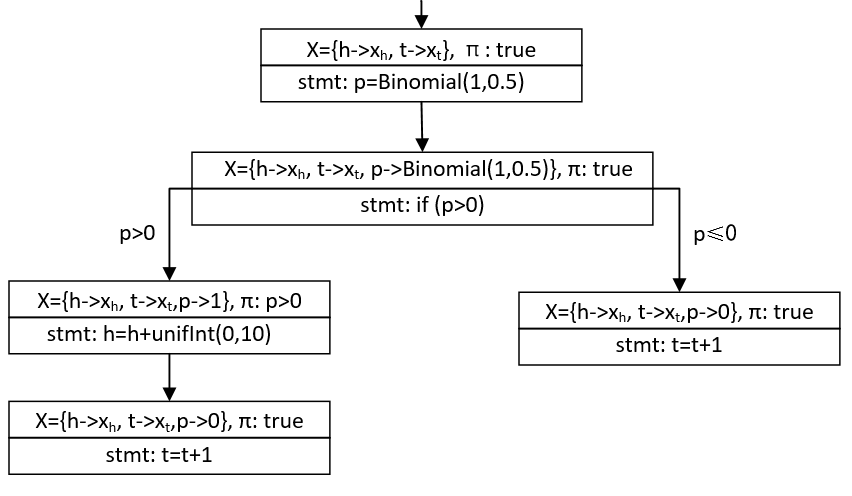
\includegraphics[scale=0.6]{img/executionTree}
	\caption{Symbolic execution tree for Example 1}
	\label{executionTree}
\end{figure}

Through a symbolic execution, we traverse the program execution tree and collect the symbolic states and path constraints, so that each path of the program execution is based on the original probability distribution. At the same time, we also do some simplification work to avoid interference from irrelevant steps(if there is an condition-branch, but neither the if-branch nor the else-branch will affect the variables related to the assertion, then the condition-branch belongs to the irrelevant setp).
Suppose the set of paths $S$ has a lower bound c on their combined path probabilities. We can still consider the estimated probability of a given assertion $\varphi$ on path set $S$ as an approximation over the whole program, and know that the contribution from the unexplored path is at most $1-c$. In this way, our method is able to handle the problem that program $P$ contains program variables and sampling variables with a wide range of distributions or even infinitely many states. 

The second step is path probability bound computation and estimating the probability of a given assertion. 
For the path set S collected above, we can analyze each path in turn, then estimate the path probability c. Each path has a series of variables and constraints. We need to estimate the probability of satisfying all constraints given the probability distributions on variables. In an overall view, it comes down to finding the satisfaction probability of the constrained system when the probability distribution of a single variable is given. Same as calculating path probability, we can seek the probabilities of assertions over variables, which can provide guaranteed interval bounds on assertion probabilities. The path condition is a conjunction of linear inequalities, so it is a convex polyhedron on R. Each variable can be regarded as a dimension of convex polyhedron.
Since the calculation of the accurate probabilities is closely related to the volume of $n$-dimensional convex polyhedron, when the dimension increases, the calculation becomes very difficult and the time complexity is high~\cite{Arora1998Proof}. Usually, the computation may fail due to the calculation or insufficient memory. 
On the premise of weighing the efficiency and accuracy of calculation, we focus on calculating lower and upper bounds of a given assertion rather than the estimated value. 

\begin{algorithm}	
	\caption{mcBoundProbability}	
	\label{mcBoundProbability}	
	\begin{algorithmic}[1]	
		\REQUIRE Polytop p=(vars, constraints), maxDepth		
		\ENSURE Probability interval $[p_1, p_2]$		
		\IF{$isABox() || maxDepth<=0$}		
		\STATE $[p1,p2]+=computeBoundingProbability()$;	
		\ENDIF  \\		
		$//$ If at least two (or more) non trivial clusters remain, then perform the decomposition.  		
		\IF{$isDecomposable(p)$}		
		\STATE dim = $selectBranchDimension()$;		
		\STATE branches= $branchAndBound(dim, nBranch)$;		
		\FOR{$b$ in branches}		
		\STATE $mcBoundProbability(b, maxDepth-1)$;		
		\ENDFOR
		\ENDIF
	\end{algorithmic}
\end{algorithm}

The calculation of path probability can be reduced to a polyhedron solving problem~\cite{Visser2012Green}. However, the solution of a convex polyhedron by linear programming is too rough. Therefore, we first decompose the convex polyhedron into several non-intersecting convex bodies~\cite{Bingsheng2020} and then add up the calculation results, as described in Algorithm~\ref{mcBoundProbability}. The input to the algorithm is $maxDepth$ and a polygon structure composed of variables and constraints. The $maxDepth$ is the maximum recurrence dept, in order to avoid infinite decomposition, with the default value $12$ in PROPER. The output is the upper bound and the lower bound of the probability.The function $isABox()$ return true if each dimension is bounded. The function $isDecomposable()$ is used to determine whether the current dimension can be decomposed. The function $selectBranchDimension()$ is based on the idea of importance sampling, selecting an unbounded or semi-bounded dimension or else it will select the maximum width dimension. The function $branchAndBound()$ is to perform the decomposition according to the selected dimension. Here, $nBranch$ is the number of segmentation, with the default value $2$. The function $computeBoundingProbability()$ is used to calculate the upper and lower bounds. 

The general idea of algorithm~\ref{mcBoundProbability} is to use multiple hypercubes to approximate a given polyhedron. The boundary of hypercube is found by continuously selecting the most influential dimension and decomposing along the selected dimension. When the boundary box is found or the maximum recursion depth exceeds $maxDepth$, the upper and lower bounds will be calculated.
The paths in the set $S$ are calculated in turn. Since there is no intersection of each path, the path probability is equal to the sum of each paths' probability. The method of calculating the assertion probability is the same as above. The assertion can be regarded as a set of constraints. Therefore, the constraint is equivalent to the disjunctive normal form of path constraint and assertion.
Let us assume that the calculation result of path probability is $[p_1,p_2]$ and assertion probability is $[p_{1'},p_{2'}]$. It indicates that the maximum $1-p_1$ path has not been explored. The upper bound of the assertion probability needs to be corrected by adding $1-p_1$. Therefore, the probability of assertion ultimately is $[p_{1'},p_{2'}-p_1+1]$


\section{Implementation and Experimental Evaluationn}
\begin{figure}[htbp]
	%\vspace{-0.5cm}  %调整图片与上文的垂直距离
	\centering %居中
	\subfigure[For termination analysis]{ %第一张子图
		%\begin{minipage}{5cm}
		\centering %子图居中
		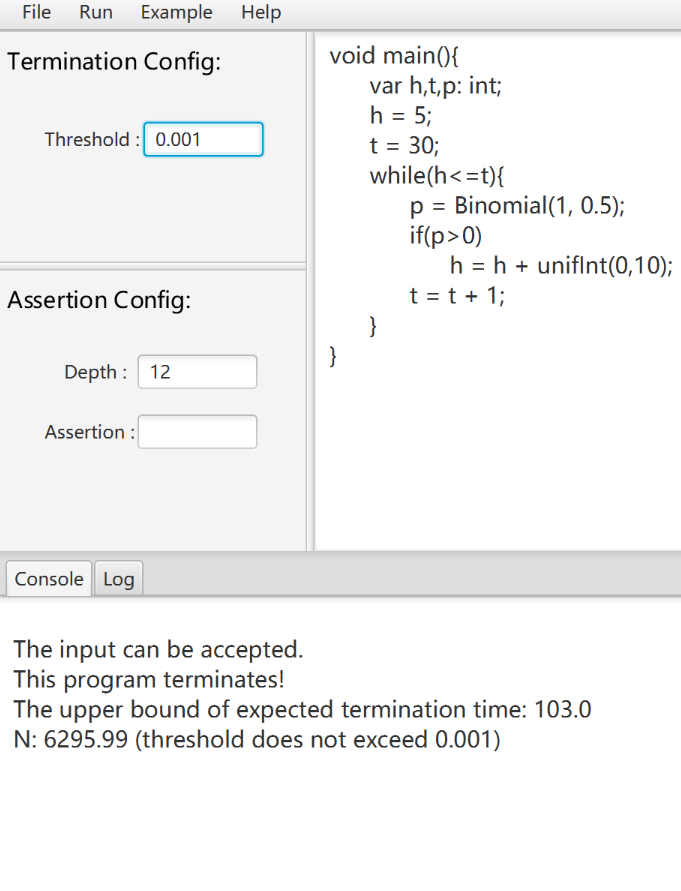
\includegraphics[scale=0.47]{img/interface1} 
		%\end{minipage}
	}\hfill
	\subfigure[For assertions analysis]{ %第二张子图
		%\begin{minipage}5cm}
		\centering %子图居中
		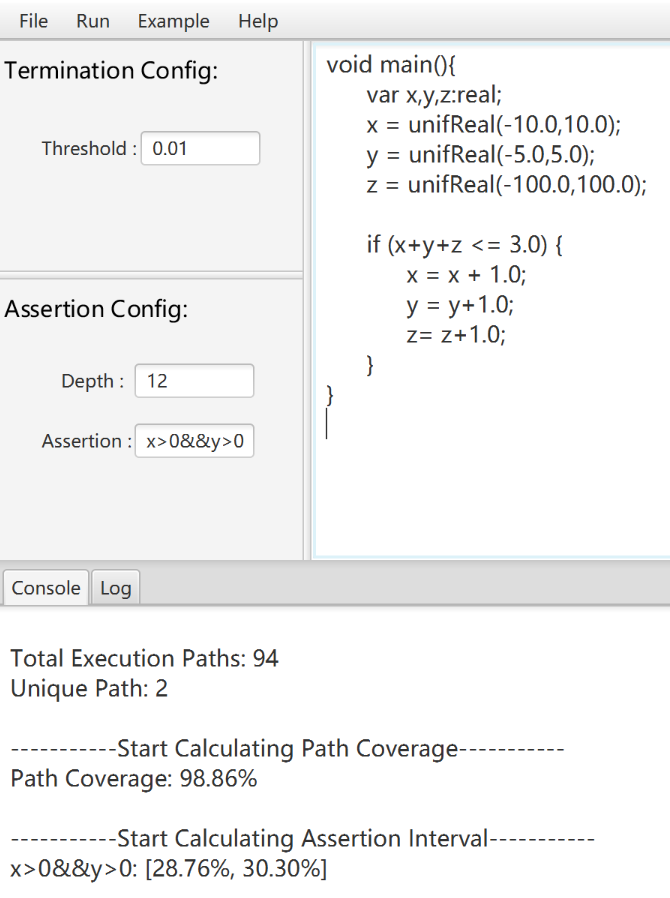
\includegraphics[scale=0.47]{img/interface2} 
		%\end{minipage}
	}
	\caption{PROPER User Interface} % %大图名称
	\label{interface} %图片引用标记
	%\setlength{\belowcaptionskip}{-1cm}   %调整图片标题与下文距离
\end{figure}
The user interface is shown in Figure \ref{interface}. Subgraph (a) is a running example of terminating analysis, and subgraph (b) is a running example of assertion analysis. At the top of the interface is a row of menu bars, which are displayed in the form of pull list, mainly including importing files, saving files, running and other functions. The concentration termination time can be set at the upper left of the interface; the recursion depth and assertion can be set at the lower left. Probabilistic programs can be written on the right, alternatively, imported from an external file. We have also built in several simple examples, you can try them. First, check the syntax specification. If it is accept, then by clicking ``Termination Analysis" or ``Assertion Analysis" in the ``Run" drop-down menu, we start the analysis process. The analysis results are displayed in the console, with two decimal places reserved.

PROPER can deal with basic probability programs with various structures, for which we have written a few simple but typical probabilistic programs, such as, single while loop(eg.Simple), multiple nesting of while loops(eg.NestedLoop), conditions statement(if) in a while loop(eg.Tortoise-Hare), conditions-branch(if-else) in a while loop(eg.RandomWalk), nesting conditions statement in a while loop(eg.Bitcoin mining) and nesting conditions-breanch statement in a while loop(eg.Gambler2).
We shall now present some experimental results of analyzing probabilistic programs using PROPER. 

\begin{table*}[htb]
	\centering
	\caption{Termination analysis}  
	\label{TerminationResult} 
	\begin{center}  
		\begin{tabular}{|l|l|l|l|l|}  
			\hline  	
			Example & $x_0$ & g($\ell_0,x_0$) & UB(P) & N (time$\leq$0.01 sec)\\ \hline  	
			Simple & $x=100$  & $6x$ & 601 & 1474.82 \\ \hline  		
			NestedLoop & $x=1, m=2$ & $1040\cdot m-1040\cdot x+208$ & 1249 & 158141.27 \\  \hline  
			Award & $bonus=0$ & $-4.0\cdot bonus+440$ & 441 &4522.28 \\  \hline  
			RandomWalk & $position=0$ & $-20\cdot position+120$ & 121 & 4695.66 \\  \hline  
			Gambler& $money=3$ & $400\cdot money+400$ & 1601 & 1506477.30 \\ \hline  		 
			Gambler2 & $money=10$ & $45.37 \cdot money+226.86$ & 908.44 & 3358.51 \\  \hline  
			Bitcoin mining & $coin=10$ & $5.32 \cdot coin$ & 54.18 & 6.39E7 \\  \hline 
			Tortoise-Hare & $h=5$, $t=30$ & $3\cdot t-3 \cdot h+27$ & 103 & 4264.27 \\  \hline  
		\end{tabular}  
	\end{center}  
\end{table*}

In Table~\ref{TerminationResult}, we display the experimental results about termination analysis, where $x_0$ means the initial value of each variable, $g(\ell_0,x_0)$ is the polynomial ranking supermartingale about the starting location, $UB(P)$ is the upper bound of expected termination time and $N$ is the bound that the probability of termination after $N$ steps shows an exponential decrement (we set the threshold to  be $0.01$).

\begin{table*}[htb]
	\centering
	\caption{Estimating the probability intervals of assertions}
	\label{AssertionsResults} 
	\begin{tabular}{|m{55pt}<{\centering} |m{130pt}<{\centering} |m{50pt}<{\centering} |m{85pt}<{\centering}|}
		%{|c |c |c |c |}
		\hline  
		Example & Assertion &  $c$ & Bounds \\ \hline
		\iffalse
		\multirow{2}{*}{carton}
		& count$\geq$5 & 0.9485 & [0.948540, 1] \\ \cline{2-4}
		& count$\geq$10 & 0.9539, & [0.000639, 0.046711] \\ \cline{2-4}
		& count$\leq$7 & 0.9549 & [0.918762, 0.963832] \\ \cline{2-4}
		& totalWeight$\geq$5.5 & 0.9386 & [0.382145, 0.453010] \\ \cline{2-4}
		& totalWeight$\geq$6 & 0.9428 & [0.246186, 0.342997]  \\ \hline
		\multirow{2}{*}{herman}
		& $ count \geq 1$ & 0.9561 & [0.581128, 0.625000] \\ \cline{2-4}
		& $ count \geq 20$ & 0.9701 & [0.000000, 0.029876]  \\ \hline
		\fi
		\multirow{3}{*}{\makecell[c]{framingham}}
		& $points \geq 10$ & 96.36\% & [13.73\%, 17.36\%] \\ \cline{2-4}
		& $pointsErr-points \geq 5$ & 96.36\% & [77.81\%, 84.93\%]  \\ \cline{2-4}
		& $points-pointsErr \geq 5$ & 96.36\% & [17.76\%, 24.68\%]  \\ \hline
		\multirow{5}{*}{\makecell[c]{sum-three}}
		& $x>5 \ \&\& \ y>0$ & 98.86\% & [15.05\%, 16.36\%]  \\ \cline{2-4}
		&  \makecell[c]{$x>0 \ \&\&\ y>0 \&\& \ z>0$} & 98.86\% & [12.56\%, 13.73\%] \\ \cline{2-4}
		& $x+y>z+10$ & 98.86\% & [44.77\%, 47.07\%] \\ \cline{2-4}
		%		& $x+y+z>8$ & 0.9886 & [0.454482, 0.475890] \\ \cline{2-4}
		& $x+y+z>100$ & 98.86\% & [1.24\%, 2.59\%]  \\ \hline
		\iffalse
		\multirow{2}{*}{ckd-epi}
		& $f -f_1\geq0.1$ & 0.9252 & [0.351632, 0.426397] \\ \cline{2-4}
		& $f_1 -f\geq0.1$ & 0.9261 & [0.387275, 0.461157]  \\ \hline
		\fi
	\end{tabular}  
\end{table*}

The results of estimating the probability intervals of assertions as shown in Table~\ref{AssertionsResults} are consistent with those in~\cite{Sankaranarayanan2013Static}. A little difference lies in the syntax of assertions. We can support the conjunction operator  ``\&\&" in PROPER that are not available before. It can analyze situations where two or more conditions are met at the same time. In the table, an assertion is a boolean expression; $c$ is the lower bound of path coverage; the column headed by Bounds gives the upper and lower bounds of the given assertion.

\section{Related Tools}
Sofware tools for the analysis of probabilistic programs has not yet received much attention. 
As far as we know, the only existing tools are ProbFuzz~\cite{DBLP:conf/sigsoft/DuttaLHM18}, PSense~\cite{DBLP:conf/atva/HuangWM18} and PSI~\cite{DBLP:conf/cav/GehrMV16}.
PSI is a symbolic inference tool that approximates the probability density function represented by a probabilistic program. 
PSense is an automated verification tool that generates tight upper bounds for the sensitivity of probabilistic programs over initial inputs.
ProbFuzz is a tool for testing probabilistic programs. 
Both the aforementioned tools do not consider termination analysis of probabilistic programs. 
For example, ProbFuzz focuses on testing rather than verification of probabilistic programs, 
PSI considers only inference and PSense solves sensitivity instead. 
Moreover, PSI/PSense requires that the input probabilistic while loop has a bounded number of loop iterations, while we can handle probabilistic loops with an unbounded number of loop iterations.

\section{Conclusion and Future Work}
Uncertainty exists in many software systems, including data analysis, stochastic algorithms and Monte Carlo simulation~\cite{HASTINGS1970Monte}. We have designed PROPER  to provide convenience and support for analyzing probabilistic programs.
PROPER is helpful to perform qualitative and quantitative analysis on the termination of probabilistic programs. It can also collect path sets with high confidence coverage and compute  probability intervals for assertions to hold in probabilistic programs.


However, we have only solved some aspects of the complex problem of probabilistic program analysis and verification. There are still many ways to improve the tool.
\begin{enumerate}
	\item Currently, PROPER only deals with linear programs. That is, it cannot handle variable multiplication, division and exponents, etc., regardless of the termination analysis or the estimation of assertion probability intervals.
	\item Non-deterministic probabilistic programs  are also not supported. PROPER requires the the behavior of the input program to be fully probabilistic, and there is no non-deterministic transitions. 
	\item In the future, we hope to find a better way to compute accurate termination time and probability intervals under the premise of ensuring high efficiency. 
\end{enumerate}

%
% ---- Bibliography ----
%
% BibTeX users should specify bibliography style 'splncs04'.
% References will then be sorted and formatted in the correct style.
%
% \bibliographystyle{splncs04}
% \bibliography{mybibliography}
%
\begin{thebibliography}{8}
\bibitem{Arora1998Proof}
Arora, Sanjeev and Lund, Carsten and Motwani, Rajeev and Sudan, Madhu and Szegedy, Mario: Proof verification and the hardness of approximation problems. Journal of the Acm \textbf{45}(3), 501--555 (1998)
\bibitem{Azuma1967}
Azuma, K.: Weighted sums of certain dependent random variables. Tohoku Mathematical Journal \textbf{19}(3), 357--367 (2010)
\bibitem{Bennett1962}
Bennett G.: Probability Inequalities for the Sum of Independent Random Variables. Journal of the American Statistical Association \textbf{57}(297), 33--45 (1962)
\bibitem{Chakarov2013Martingales}
Chakarov A., Sankaranarayanan S.: Probabilistic Program Analysis with Martingales. International Conference on Computer Aided Verification Springer, Berlin, Heidelberg, (2013)
\bibitem{kris2016termination}
Chatterjee, K., Fu, H., Goharshady, A.K.: Termination Analysis of Probabilistic Programs through Positivstellensatz's. In: CAV, pp. 3--22 (2016)
\bibitem{cha2015algorithmic}
Chatterjee, K., Fu, H., Novotn\'{y}, P., Hasheminezhad, R.: Algorithmic analysis of
qualitative and quantitative termination problems for affine probabilistic programs. In: POPL, pp. 327--342 (2016)
\bibitem{Dav2016Design}
David Tolpin, Jan-Willem van de Meent, Hongseok Yang, and FrankWood: Design and Implementation of Probabilistic Programming Language Anglican. In: IFL. ACM, 6:1–6:12. (2016)
\bibitem{DBLP:conf/sigsoft/DuttaLHM18}
Dutta S., Legunsen O., Huang Z., et al.: Testing probabilistic programming systems. the 26th ACM Joint Meeting. (2018)
\bibitem{tran2016edward}
Dustin Tran and Alp Kucukelbir and Adji B. Dieng and Maja Rudolph and Dawen Liang and David M. Blei: Edward: A library for probabilistic modeling, inference, and criticism. (2016) \doi{1610.09787}
\bibitem{Farkas1894}
Farkas J.: A fourier-f\'{e}le mechanikai elv alkalmaz\'{a}sai (Hungarian). Mathematikai\'{e}s Term\'{e}szettudom\'{a}nyi \'{E}rtesit\''{o} \textbf{12}, 457--472 (1894)
\bibitem{HASTINGS1970Monte}
HASTINGS and W., K.: Monte Carlo sampling methods using Markov chains and their applications. Journal of the Acm, 97--109 (1970)
\bibitem{Hoeffding1963}
Hoeffding W.: Probability Inequalities for Sums of Bounded Random Variables. Encyclopedia of Statistical Sciences. American Cancer Society (2004)
\bibitem{DBLP:conf/atva/2018}
Huang Z., Wang Z., Misailovic S.: PSense: Automatic Sensitivity Analysis for Probabilistic Programs. Automated Technology for Verification and Analysis - 16th International
Symposium. (2018)
\bibitem{Hermanns2013Probabilistic}
L.M.F. Fioriti, H. Hermanns: Probabilistic termination : Soundness, completeness, and compositionality. In: POPL, pp. 489--501 ACM(2015)
\bibitem{McDiarmid1998Concentration}
McDiarmid C.: Concentration. In Probabilistic Methods for Algorithmic Discrete Mathematics. Algorithms in combinatorics \textbf{16}, 195--248 (1998)
\bibitem{Noah2008language}
Noah D Goodman, Vikash K Mansinghka, Daniel Roy, Keith Bonawitz, and Joshua B Tenenbaum: Church: a language for generative models. In: UAI, pp. 220--229. AUAI Press (2008)
\bibitem{Noah2014language}
Noah D Goodman and Andreas Stuhlmüller: The Design and
Implementation of Probabilistic Programming Languages. (2014)
\bibitem{Sankaranarayanan2013Static}
Sankaranarayanan, Sriram and Chakarov, Aleksandar and Gulwani, Sumit.: Static Analysis for Probabilistic Programs: Inferring Whole Program Properties from Finitely Many Paths. acm sigplan notices \textbf{48}(6), 447--458 (2013)
\bibitem{DBLP:conf/cav/2016-1}
Swarat Chaudhuri and Azadeh Farzan. Vechev: {PSI:} Exact Symbolic Inference for Probabilistic Programs. Computer Aided Verification - 28th International Conference, 62--83 (2016)
\bibitem{DBLP:conf/cav/GehrMV16}
Timon Gehr and Sasa Misailovic and Martin T. Vechev: {PSI:} Exact Symbolic Inference for Probabilistic Programs. Computer Aided Verification - 28th International Conference, 62--83 (2016)
\bibitem{Turing1936On}
Turing A.: On Computable Numbers, with an Application to the Entscheidungsproblem. Alan Turing His Work \& Impact, 13--115 (2013)

\end{thebibliography}
\end{document}
